\documentclass[10pt, letter]{article}
\newcommand{\doctitle}{%
CS 4649/7649: RIP - Robot Intelligence - Planning}
\newcommand{\bigO}{\ensuremath{\mathcal{O}}}
\usepackage{graphicx}
\usepackage{float}
\usepackage{comment}
\usepackage{fancyvrb}
\usepackage{booktabs}
\usepackage[usenames,dvipsnames]{color}
\usepackage[center]{caption}
\usepackage{algorithm}
\usepackage[T1]{fontenc}
\usepackage[noend]{algpseudocode}
\usepackage{algorithm}
\usepackage[margin=1in]{geometry}
\usepackage[usenames,dvipsnames]{color}
\usepackage{hyperref}
\usepackage{xcolor}
\usepackage{amsmath}
\hypersetup{
  colorlinks,
  citecolor=Violet,
  linkcolor=Black,
  urlcolor=Blue}
%------------------------Included every possible package we might need ------------------------%
\begin{document}
\title{\textbf{\doctitle} \\\textsc{Project 1: Classical Sokoban Planner}}
  \author {Arvind Krishnaa Jagannathan, Zheng Yong, Luis Gustavo, Zhengyi Hu}%Others please check your names here
   \date{}
\maketitle

\section{Pre-Project: Towers of Hanoi}
%Assigned to Arvind%
\subsection*{Planners Used}
The two classical planners which we are using for the Towers of Hanoi problem are the Blackbox planner \cite{kautz1998blackbox} (downloaded from \url{http://www.cs.rochester.edu/~kautz/satplan/blackbox/blackbox-download.html}) and the FF planner \cite{hoffmann2001fast} (downloaded from \url{http://fai.cs.uni-saarland.de/hoffmann/ff/FF-v2.3.tgz}). The definition of the Towers of Hanoi domain, as well as the representation of the initial state of the problem (from Figure \ref{fig1}) are in the corresponding PDDL files, namely \textit{hanoi-domain.pddl} and \textit{hanoi-3.pddl}.

\begin{figure}[h!]
  \centering
    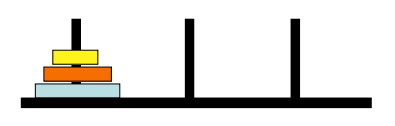
\includegraphics[scale = 0.3]{images/hanoi1}
    \caption{Towers of Hanoi with 3 disks}
  \label{fig1}
\end{figure}

\subsection{Questions}
\subsubsection*{1. Explain the method by which each of the two planners finds a solution}
\textbf{BlackBox}- The Blackbox planning algorithm essentially represents the PDDL representation of a problem as a set of Boolean satisfiability problems (SAT), which are then solved using a variety of SAT solvers (such as satz, walksat and chaff) to produce a plan.
In order to construct the SAT problem, Blackbox uses the \textsc{GraphPlan} algorithm to construct a plan graph for the given problem representation. This plan graph is then ``translated'' to the SAT problem representation. This is outlined briefly below:

The \textsc{GraphPlan} algorithm works by constructing a planning graph out of a \textsc{Strips} representation, which will propagate actions/operators across different ``layers'' along with their ``mutex'' pre-conditions. So at every stage there will be a list of actions, which have mutually exclusive pre-conditions. The plan generated by \textsc{GraphPlan} will be a sub-graph of the plan graph such that, all the conditions of the initial and final state are incorporated without there being any ``conflicting'' actions. As described by Kautz et. al \cite{kautz1996encoding}, each state in this solution graph can be encoded into propositional logic. This can be done by adding propositions of the form,
\begin{center}
$Precondition_i$ $\implies$ $Action_j$
\end{center}
At each layer of the solution sub-graph, clauses/fluents can be resolved away to result in a compact propositional logic representation of the plan graph. This list of proposition corresponds to the ``translation'' of the plan graph into a SAT problem. Then any available SAT solver can be applied on this problem which (although NP-complete in theory) with reasonable assumptions be completed in exponential time. ($O(n^3)$)

\textbf{FF Planner} - The fast-forward planning algorithm utilizes \textsc{GraphPlan} as an admissible (and informed) heuristic to solve the planning problem using a search algorithm across the set of permissible states in the state space. FF planner works as follows: it sets up a relaxed solvable sub-problem ($S\prime$) of the original problem ($S$).Then \textsc{GraphPlan} is applied on the relaxed sub-problem; the length of the solution plan sub-graph is then treated as a heuristic to guide the state space search algorithm for a plan to the original problem. This takes into account the positive interactions between various facts in the problem.

FF uses the enforced hill climbing algorithm to search for valid solutions. Using the length of the relaxed \textsc{GraphPlan} solution as a heuristic, the enforced hill climbing algorithm evaluates the direct successors of a search state S. Until a state ($S\prime$) is found with a better heuristic evaluation than $S$, the search goes one step further.

Thus in summary both \textit{\textbf{FF}} and \textit{\textbf{Blackbox}} algorithms use the \textsc{GraphPlan} algorithm, however \textit{Blackbox} uses it in a more direct way, to set up the SAT problem. In \textit{FF}, \textsc{GraphPlan} is used simply as a heuristic measure for the enforced hill climbing algorithm.
\subsubsection*{2. Which planner was fastest?}
Both the algorithms were run on the same Linux box, and using the \textit{time} command the time taken for them to produce plans were measure. Clearly the \textbf{FF} algorithm was the fastest among the two, with the following time measures \\
\begin{itemize}
\item FF - 0.004s
\item Blackbox - 0.011s
\end{itemize}
This shows that \textbf{FF} is 2.75 times faster than \textbf{Blackbox}. This is pretty much expected from theory since the time complexity for each of the algorithms are,
\begin{center}
	O(\textit{Blackbox}) = O(\textsc{GraphPlan'}) + O(\textit{SAT Solver})\\
	O(\textit{FF}) = O(\textsc{GraphPlan}) + O(\textit{Enforced Hill Climbing})\\
	O(\textit{Enforced Hill Climbing}) = O(iterations x successors),\\
	O(\textit{SAT Solver}) = O($2^n$)
\end{center}
Clearly the SAT solver's exponential time complexity, as well as the time complexity of the complete \textsc{GraphPlan} algorithm for \textit{Blackbox} vs. that of the relaxed \textsc{GraphPlan} as well as that of \textit{Enforced Hill Climbing} for the \textit{FF} make it obviously slower than FF; this has been shown by using the towers of hanoi state and domain PDDL description multiple times (to get an average measure) with Blackbox and FF.
\subsubsection*{3. Explain why the winning planner might be more effective on this problem}
Its pretty obvious that the length of a plan in case of the Towers of Hanoi problem are a similar order of magnitude as that of the total number of states ($2^n - 1$ steps and $3^n$ states). In case of the \textbf{FF} planner, \textsc{GraphPlan} is used only as a heuristic and that too for a relaxed subset. \textit{FF}'s major component is the local-search algorithm, which means it does not have to necessarily traverse all the states in order to obtain a solution.

\textit{Blackbox} on the other needs to explicitly construct the mutex graph for every level until a solution is obtained. In case the state space is large (like 10 disks in the Towers of Hanoi problem), the construction of a complete plan graph is memory prohibitive and will not be effective on larger instances of this problem (it actually does not give plans for even 6 disks on my machine after 1 minute of execution). Another major issue with \textit{Blackbox} is that several levels of the \textsc{GraphPlan} algorithm may lead to the same set of SAT problems, which will remain unsatisfiable. \textit{Blackbox} is bound to be less effective in similar large state problems, since it seems to perform the same computation multiple times.

%-----------------------------------End of Problem 1 ---------------------------------------------%

\section{Project Part I: Sokoban PDDL}
%Assigned to Luis%

\begin{figure}[h]
  \centering
    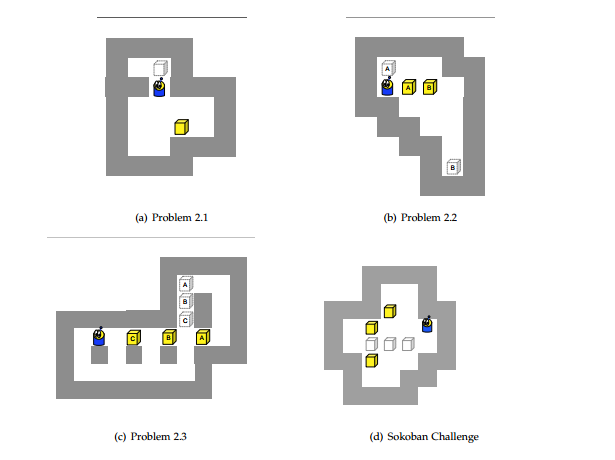
\includegraphics[scale = 0.3]{images/sokoban}
    \caption{Sokoban Problems}
  \label{fig2}
\end{figure}

\subsection{Questions}
\subsubsection*{1. Show successful plans from at least one planner on the three Sokoban problems in Figure \ref{fig2}
(1-3). The challenge problem is optional}
\subsubsection*{2. Compare the performance of two planners on this domain. Which one works better? Does this
make sense, why?}
\subsubsection*{3. Clearly PDDL was not intended for this sort of application. Discuss the challenges in expressing geometric constraints in semantic planning}
\subsubsection*{4. In many cases, geometric and dynamic planning are insufficient to describe a domain. Give
an example of a problem that is best suited for semantic (classical) planning. Explain why a
semantic representation would be desirable}

%------------------------------------End of Problem 2 -------------------------------------------------%

\section{Project Part II: Sokoban Planner}
%Assigned to James and Stango%
\subsection{Questions}
\subsubsection*{1. Give successful plans from your planner on the Sokoban problems in Figure \ref{fig2} and any others}
\subsubsection*{2. Compare the performance of your planner to the PDDL planners you used in the previous
problem. Which was faster? Why?}
\subsubsection*{3. Prove that your planner was complete. Your instructor has a math background: a proof ``is
a convincing argument.'' Make sure you address each aspect of completeness and why your
planner satisfies it. Pictures are always welcome.}
\subsubsection*{4. What methods did you use to speed up the planning? Give a short description of each method
and explain why it did or didn't help on each relevant problem}

%---------------------------------End of Problem 3 ----------------------------------------------------%

\section{Post-Project: Towers of Hanoi Revisited}
%Assigned to Arvind%
Constructing a PDDL representation for the N-disk towers of hanoi is pretty simple by utilizing the following simple structures, for initializing the problem state
\begin{enumerate}
\item Each disk labeled $D_i$ is smaller than a disk labeled $D_{i+1}$. That is \texttt{(smaller $d_i$ $d_{i+1}$)}.
\item Every disk is smaller than each of the three poles (by definition).
\item The smallest disk (i.e., D1), and the two other poles (P1 and P2) are clear.
\item Every disk $D_i$ is \emph{on} the disk $D_{i+1}$. The largest disk D10, is \emph{on} the pole P3.
\item Every element $D_i$ is a disk
\end{enumerate}
The goal state is simply a conjunction (\textsc{And}-ing) of all the states mentioned in Step 4 above, except that the largest disk D10, is \emph{on} the pole P1.

The corresponding PDDL representations for the 6 disk and 10 disk towers of hanoi problem are present in the files ``hanoi-6.pddl'' and ``hanoi-10.pddl''.

Both \textbf{FF} and \textbf{Blackbox} planners were applied onto the PDDL representations, however only \textit{FF} was able to produce valid plans for the 6 disk and 10 disk problem. \textit{Blackbox} was unable to produce any results, due to relatively large nature of the state-space (I halted execution after 1 minute since the blackbox executable started running).

\subsection{Questions}
\subsubsection*{1. Give successful plans from at least one planner with 6 and 10 disks}
The plan for the towers of hanoi problem with 6 disk, generated by \textit{FF} is as follows:\\
\begin{verbatim}
step    0: MOVE-DISK D1 D2 P2
        1: MOVE-DISK D2 D3 P1
        2: MOVE-DISK D1 P2 D2
        3: MOVE-DISK D3 D4 P2
        4: MOVE-DISK D1 D2 D4
        5: MOVE-DISK D2 P1 D3
        6: MOVE-DISK D1 D4 D2
        7: MOVE-DISK D4 D5 P1
        8: MOVE-DISK D1 D2 D4
        9: MOVE-DISK D2 D3 D5
       10: MOVE-DISK D1 D4 D2
       11: MOVE-DISK D3 P2 D4
       12: MOVE-DISK D1 D2 P2
       13: MOVE-DISK D2 D5 D3
       14: MOVE-DISK D1 P2 D2
       15: MOVE-DISK D5 D6 P2
       16: MOVE-DISK D1 D2 D6
       17: MOVE-DISK D2 D3 D5
       18: MOVE-DISK D1 D6 D2
       19: MOVE-DISK D3 D4 D6
       20: MOVE-DISK D1 D2 D4
       21: MOVE-DISK D2 D5 D3
       22: MOVE-DISK D1 D4 D2
       23: MOVE-DISK D4 P1 D5
       24: MOVE-DISK D1 D2 D4
       25: MOVE-DISK D2 D3 P1
       26: MOVE-DISK D1 D4 D2
       27: MOVE-DISK D3 D6 D4
       28: MOVE-DISK D1 D2 D6
       29: MOVE-DISK D2 P1 D3
       30: MOVE-DISK D1 D6 D2
       31: MOVE-DISK D6 P3 P1
       32: MOVE-DISK D1 D2 D6
       33: MOVE-DISK D2 D3 P3
       34: MOVE-DISK D1 D6 D2
       35: MOVE-DISK D3 D4 D6
       36: MOVE-DISK D1 D2 D4
       37: MOVE-DISK D2 P3 D3
       38: MOVE-DISK D1 D4 D2
       39: MOVE-DISK D4 D5 P3
       40: MOVE-DISK D1 D2 D4
       41: MOVE-DISK D2 D3 D5
       42: MOVE-DISK D1 D4 D2
       43: MOVE-DISK D3 D6 D4
       44: MOVE-DISK D1 D2 D6
       45: MOVE-DISK D2 D5 D3
       46: MOVE-DISK D1 D6 D2
       47: MOVE-DISK D5 P2 D6
       48: MOVE-DISK D1 D2 P2
       49: MOVE-DISK D2 D3 D5
       50: MOVE-DISK D1 P2 D2
       51: MOVE-DISK D3 D4 P2
       52: MOVE-DISK D1 D2 D4
       53: MOVE-DISK D2 D5 D3
       54: MOVE-DISK D1 D4 D2
       55: MOVE-DISK D4 P3 D5
       56: MOVE-DISK D1 D2 D4
       57: MOVE-DISK D2 D3 P3
       58: MOVE-DISK D1 D4 D2
       59: MOVE-DISK D3 P2 D4
       60: MOVE-DISK D1 D2 P2
       61: MOVE-DISK D2 P3 D3
       62: MOVE-DISK D1 P2 D2
\end{verbatim}
Clearly it has $2^6 - 1$ = 63 steps in the plan. Now the problem with 10 disks will have a plan of $2^10 - 1$ = 1023 steps. The \textit{FF} planner produces a valid plan with 1023 steps, but for the lack of space it is not produced here. The plan is present under the resources directory as ``hanoi-10-solutions''.

\subsubsection*{2. Do you notice anything about the structure of the plans? Can you use this to increase the
efficiency of planning for Towers of Hanoi? Explain}
One observation from the three plans generated (3, 6 and 10 disks) is that whenever there are odd number of initial disks, then the top most disk is moved onto the ``destination'' pole, and when there are even number of initial disks, then the top most disk is moved onto the ``middle'' pole.

Another noticeable aspect of the problem is that the towers of hanoi can be viewed as a simple recursive problem of moving the smaller $n-1$ disks from $P3$ to $P2$ then moving the largest disk from $P3$ to $P1$ followed by moving the $n-1$ disks from $P2$ to $P1$. This can be empirically verified - at every $(2^N - 1)^{th}$ step, if the initial number of disks $n$ are odd, then there will be $N-1$ disks on P2 and largest disk will be on P1. If the initial number of disks $n$ are even, then there will be $N-1$ disks on $P3$ and the largest will be on $P2$. Of course here, $0<N<=n$.

Thus the entire plan can be represented recursively (and efficiently) as: 
\begin{algorithm}
  \caption{Towers of Hanoi recursive definition}
  \begin{algorithmic}[1]
    \Function{Hanoi-Solver}{$N, P3, P2, P1$}
    \Comment{Move N disks from P3 to P1 (using P2 as intermediate)}
		\State \Call{Hanoi-Solver}{$N-1, P3, P1, P2$}
		\State \Call{Move}{$1, P3, P1$} \Comment{Move the largest disk from P3 to P1}
	  	\State \Call{Hanoi-Solver}{$N-1, P2, P3, P1$}
    \EndFunction
  \end{algorithmic}
\end{algorithm}

Thus this is a bottom-up approach in constructing a plan. All one needs to define are the ``macro'' propositions \textsc{Hanoi-Solver} and \textsc{Move} (which is applied when there is just the largest disk remaining on $P3$). The planner can then use this base condition (a.k.a ``macro'' proposition) and basically ``un-wind'' the call stack to generate sub-plans. The correct plan is then obtained by simply reversing the ``popped'' elements of the call stack.


\subsubsection*{3. In a paragraph or two, explain a general planning strategy that would take advantage of
problem structure. Make sure your strategy applies to problems other than Towers of Hanoi.
Would such a planner still be complete?}

A general recursive algorithm takes advantage of whenever there is a possibility of breaking down a problem into multiple smaller, but similarly structured problems, each if solved (and possibly in parallel if there is sufficient independence) can be ``combined'' to get the solution to the original problem. The generic recursive algorithm is:

\begin{algorithm}
  \caption{Recursive Planner}
  \begin{algorithmic}[1]
    \Function{Recursive-Planner}{$Prob_N$}
    \Comment{Solve a sub-problem}
    		\If{Some Terminal Condition}
			\State \Call{Terminal-Operation}{$Prob_1$} \Comment{Some constant terminal operation}
		\EndIf
		\State \Call{Recursive-Planner}{$Subset(Prob_N)$}
    \EndFunction
  \end{algorithmic}
\end{algorithm}

There are a whole class of problems to which a recursive planner can be applied. For instance, this algorithm can be used in large scale map navigation problems, where loading an entire terrain in one go may be memory prohibitive.

There are two conditions for a planner to be complete,
\begin{enumerate}
\item \textbf{Produces a plan if there is one}: The recursive planner relies on all the sub-goals to complete their execution (or the recursion stack to be empty). So in case all the sub-goals reach their respective terminating condition, then all of them will reach completion (this is from an execution standpoint - different from the notion of completeness). If all the individual problems finish, then the top-level problem, which is basically a composition of these sub-problems will also produce a valid plan.

However, it is possible that even though the entire problem has a solution, one of the sub-problems may never reach completion -- this would cause the original problem to not produce a plan. Hence it cannot always be guaranteed that the planner produces a plan if there is a valid one.

\item \textbf{Reports that there is no plan if there is none}: The same sub-problem non-termination issue exists here as well. In case one of the sub-problems gets ``stuck'', there is no way for the original problem to terminate reporting that there is no plan. 
\end{enumerate}

However, if some sort of a terminating ``\textit{parameter}'' can be used to force the sub-problems to halt/report no solution. In such a case the ``stack overflow'' issue will be resolved and both the conditions of completeness will be met. Basically, we need to ensure that the sub-problems will be forcibly terminated which will ensure that the main problem will always terminate as well!

%----------------------------------End of Problem 4 ----------------------------------------------------%

\bibliographystyle{unsrt}
\bibliography{myrefs}
\end{document}